%% Template for a preprint Letter or Article for submission
%% to the journal Nature.
%% Written by Peter Czoschke, 26 February 2004
%%

\documentclass[%
%superscriptaddress,
%groupedaddress,
%unsortedaddress,
%runinaddress,
%frontmatterverbose, 
%preprint,
showpacs,
%preprintnumbers,
%nofootinbib,
%nobibnotes,
%bibnotes,
 amsmath,amssymb,
 aps,
 twocolumn,
 prl,
 reprint,
%pra,
%prb,
%rmp,
%prstab,
%prstper,
floatfix,
]{revtex4-1}

\usepackage{graphicx}% Include figure files
\usepackage{dcolumn}% Align table columns on decimal point
\usepackage{bm}% bold math
%\usepackage{lineno}
\usepackage{color}
\usepackage{acronym}
\usepackage{multirow}
\usepackage{tabularx}
\usepackage{hyperref}
%\addbibresource{references.bib}
%\linenumbers % Commence numbering lines
%\usepackage{hyperref}% add hypertext capabilities
%\usepackage[mathlines]{lineno}% Enable numbering of text and display math
%\linenumbers\relax % Commence numbering lines
\hypersetup{
%--- fill inside borders ---
  colorlinks=true,        % false: boxed links; true: colored links
  linkcolor=black,         % color of internal links
  citecolor=cyan,         % color of links to bibliography
}

%% make sure you have the nature.cls and naturemag.bst files where
%% LaTeX can find them

%\bibliographystyle{authortitle}

%% Notice placement of commas and superscripts and use of &
%% in the author list

%\author{Hunter Gabbard$^{1}$, Ik Siong Heng$^1$, Chris Messenger$^1$, \\
%    Francesco Tonolini$^2$, \& Roderick Murray-Smith$^2$}

%% ----- comment commands for each of us
\newcommand{\chris}[1]{\textbf{\textcolor{green}{CHRIS: #1}}}
\newcommand{\francesco}[1]{\textbf{\textcolor{red}{FRANCESCO: #1}}}
\newcommand{\hunter}[1]{\textbf{\textcolor{blue}{HUNTER: #1}}}
\newcommand{\siong}[1]{\textbf{\textcolor{cyan}{SIONG: #1}}}
\newcommand{\rod}[1]{\textbf{\textcolor{yellow}{ROD: #1}}}

\begin{document}

\preprint{APS/123-QED}

\title{Estimating Bayesian Parameter Estimation Using Conditional Variational Autoencoders}

\author{Hunter Gabbard$^1$}
 \email{Corresponding author: h.gabbard.1@research.gla.ac.uk}
\author{Ik Siong Heng$^1$}
\author{Chris Messenger$^1$}
\author{Francesco Tonolini$^2$}
\author{\& Roderick Murray-Smith$^2$}

\affiliation{
 SUPA, School of Physics and Astronomy$^1$, \\
 School of Computing Science$^2$, \\
 University of Glasgow, \\
 Glasgow G12 8QQ, United Kingdom \\
}

\date{\today}

\maketitle

\acrodef{BBH}[BBH]{binary black hole}
\acrodef{SNR}[SNR]{signal-to-noise ratio}
\acrodef{PSD}[PSD]{power spectral density}
\acrodef{FFT}[FFT]{fast Fourier transform}
\acrodef{CNN}[CNN]{convolutional neural network}
\acrodef{ROC}[ROC]{receiver operator characteristic}

%
% Introductory paragraph describing the content of the letter
%
\textbf{
With the beginning of the Laser Interferometer Gravitational wave Observatory's 
(LIGO) and Virgo's third observation run well under way, we are now in an era 
where gravitational wave (GW) detection is commonplace \cite{PhysRevLett.116.061102,
PhysRevX.6.041015,PhysRevLett.119.161101}. As the sensitivity of 
both detectors increases, we will see more many more detections on a weekly 
and even daily basis.  The current method used to estimate the parameters of 
gravitational wave events is done using a form of Bayesian inference \cite{1409.7215}. Although 
effective, Bayesian inference is a computationally expensive method which can 
take of order hours to weeks to complete when applied to a single GW event. We 
propose the use of a conditional variational autoencoder (CVAE) as a 
computationally inexpensive alternative to this approach \cite{1904.06264,1812.04405}. Here we show that 
a CVAE can return posterior estimates for any parameter of a detected GW 
event on the order of less than $1s$, an immense speed-up over current 
inference techniques.}

%
% Set up parameter estimation problem
%
In the standard Bayesian GW inference approach, we assume that we are given 
some observed waveform which is buried in noise. In order to ensure that there is 
equal power accross all frequency bins of our signal, we ensure that 
the noise is whitened Gaussian noise. We whiten using 
a single detector (H1) power spectrum density derived from the Advanced 
LIGO design sensitivity curves \cite{2016LRR....19....1A}.  Given a noisy GW waveform, we would like 
to find an optimal procedure for retrieving some finite set of unknown GW parameters \cite{Jaranowski2012}
. Our procedure should be able to give us an accurate estimate 
of the parameters of our observed signal, while also accounting for the uncertainty 
which arises from having multiple noise realizations of our observed data able to 
be mapped to one parameter estimate.

%
% Describe Bayes Theorem
%
According to Bayes Theorem \cite{Bayestheorem}, a posterior for a set of GW parameters can be described 
by the following expression:

\begin{equation}
    p(\theta|x) = \frac{p(x|\theta) * p(\theta)}{p(x)},
\end{equation}

where $p(\theta|x)$ is the probability of the parameters given observed data, 
$p(x|\theta)$ is the probability of the observed data given the parameters, $p(\theta)$ 
is the prior we put on our parameter distribution and $p(x)$ is the probability of our data. 
We typically assume that $p(x)$ is a constant, $1$, which then reduces to the following equation:

\begin{equation}
    p(\theta|x) \propto p(x|\theta) * p(\theta),
\end{equation}

where $p(\theta|x)$ is the posterior, $p(x|\theta)$ is the likelihood and $p(\theta)$ is the prior. 
For this study, we assume that the noise is stationary with zero mean and some constant variance 
in each detector. Small changes in the power spectrum density over time are not considered in this analysis. 

%
% Describe nested sampling algorithm
%
There are several algorithms which may be used to sample from the posterior distribution 
of astrophysical GW source parameters. The algorithm which is used in our studies is 
the nested sampling algorithm. Nested sampling takes a multi-dimensional evidence 
integral calculation (fully marginalized likelihood) and transforms it into a more 
manageable 1-D integral. Where the fully marginalized likelihood is equivalent to taking 
the integral of the likelihood and multiplying it by the prior \cite{1409.7215}.

The first step of the nested sampling algorithm starts by generating an initial 
set of live points made from the prior distribution. The likelihood for each point 
is calculated and the point with the lowest likelihood is removed. The removed sample 
is then replaced with a new sample which has a higher likelihood. This cycle repeats 
itself until a predefined stopping threshold is achieved \cite{1409.7215}
. Samples 
from the posterior may be drawn by randomly selecting from both all current 'live' 
points and all previously removed 'live' points. 

%
% discuss codebase which we use to generate waveforms, sampling frequency, and paramter space
%
The codebase which we use to do the Bayesian inference analysis is the Bilby inference library \cite{1811.02042}
. Our waveforms have a duration of 1 second, sampling frequency 
of 256Hz, fixed right ascension ($\alpha$), declination ($\delta$), inclination angle 
($\theta_j$), polarization angle ($\psi$) and a spin of zero. We allow 5 
parameters to vary: component masses $m_1$ and $m_2$, luminosity distance, time of coalescence and phase, 
where phase is marginalized out. The waveform model used is 
\texttt{IMRPhenomPv2} \cite{1809.10113} with a minimum cutoff frequency of 20Hz.

%
% Discuss priors that we use
%
The priors we choose for the analysis are all fixed except for the component masses, phase, distance 
and time of coalescence. The prior on both component masses range from 
$35 - 50$ solar masses, the phase prior ranges from $0 - 2\pi$, the distance prior ranges from $1\textrm{Gpc} - 3\textrm{Gpc}$, and 
the time of coalesence prior ranges from $1126259642.4 - 1126259642.6$. The nested sampling algorithm is run 
using 1000 live points and has a predefined stopping criteria of $0.1$. The sampler takes 
$\mathcal{O}(3 \: \textrm{minutes})$ to converge.

%
% Conclude bilby section
% 
After the nested sampler has converged, we draw samples and produce a posterior on the 
astrophysical GW source parameters we are trying to estimate. These samples will be 
used as our benchmark when assessing the efficiency of our machine learning approach. 
We will now investigate whether we can reproduce the results from Bilby using CVAEs. 
   

%
% Intro to machine learning section
%
Machine learning has featured prominently in many areas of gravitational wave research over the last few years.
These techniques have shown to be particularly useful
in signal detection \cite{PhysRevLett.120.141103,GEORGE201864,1904.08693}, glitch classification \cite{1706.07446,0264-9381-34-6-064003} and
earthquake prediction \cite{Coughlin_2017}. Recently, a type of neural network
called conditional variational autoencoders was shown to perform exceptionally well 
when applied towards computational imaging inference \cite{1904.06264}. It is this network 
that we base our machine learning inference algorithm off of.

%
% What is an autoencoder?
%
Conditional variational autoencoders are a form of variational autoencoders 
which are conditioned on an observation. The autoencoders from which variational autoencoders 
are derived are typically used 
for problems involving image reconstruction and attempt to reproduce a  
given input. An autoencoder is composed of two neural networks, an encoder 
and a decoder \cite{LIOU20083150}. The encoder network takes as input an image, then converts 
the input image into a (typically) lower dimensional space, what is also known as the {\it{latent space}}. 
The latent space is then fed as input to the decoder network 
which generates as output a reconstruction of the original input
image to the encoder network. Through training, we hope to learn a latent space which will 
take on the most important properties of our input training samples.  

%
% What is a variational autoencoder?
%
One of the few failings of an autoencoder is that they are only able to return one 
output for any one given input. In order to produce variable estimates for 
one given input, we need to utilize what is known as a variational autoencoder \cite{1812.04405}.
A variational autoencoder is also composed of both an encoder and a decoder network. 
The primary difference between a variational autoencoder and an autoencoder concerns the method by which the 
latent space is produced. In our variant of the variational autoender, the mean ($z_{\mu}$) and the log squared 
of the standard deviation ($z_{\log{(\sigma^{2})}}$) of the output of the encoder is calculated. We then multiply 
the log squared of the standard deviation by a random unit Gaussian distribution ($\epsilon(0,1)$) which is 
of the same dimension as that of the latent space.

\begin{equation}
    z = z_{\mu} + z_{\log{(\sigma^{2})}} \cdot \epsilon(0,1).\label{eq:z_calc}
\end{equation}

$\log{(\sigma^{2})}$ is then summed together 
with the mean to produce the latent space $z$ (Eq. \ref{eq:z_calc}). The latent space is given as input 
to the decoder network, which attempts to reconstruct the given input to 
the encoder network. We use fully-connected layers in 
both the decoder and the encoder networks.

%
% How does our 3-network set-up work?
%
For this study, we will use a combination of three networks; two encoder networks ($\textrm{E}_1$, $\textrm{E}_2$) 
and one decoder network (D). The decoder network takes as input a set of latent space 
$z$ predictions from one of the encoder networks. The decoder network samples from 
the posterior by producing $x_{\mu}$/$x_{\log{(\sigma^{2})}}$ predictions on our parameters 
and then applying a random unit variant Gaussian distribution $\epsilon(0,1)$.

\begin{equation}
    x_{\textrm{samp}} = x_{\mu} + x_{\log{(\sigma^{2})}} \cdot \epsilon(0,1).\label{eq:x_calc}
\end{equation}

$\textrm{E}_1$ takes as 
input a set of GW signals and produces a latent space vector $z^1$, while $\textrm{E}_2$ 
takes as input both a set of GW signals and their associated source parameters 
and produces a another latent space vector $z^2$.

\begin{figure}
    \includegraphics[width=\columnwidth]{images/network_setup.png}
    \caption{\label{fig:network_config} This figure illustrates our neural network 
    training/testing operations. During training, a training set of GW signals ($y$) 
    and their corresponding true parameters ($x$) are given as input to encoder 
    networks $\textrm{E}_1$ and $\textrm{E}_2$. The KL divergence (Eq. \ref{eq:kl}) 
    is computed between mean latent space predictions from both encoder networks ($z^1_{\mu},z^2_{\mu}$)
    . $z^2_{\mu}$ is then summed togther with $z_{\log{(\sigma^{2})}} \cdot \epsilon(0,1)$ 
    and given as input to the decoder network. The decoder network predicts $x_{\mu}$ 
    and compares $x_{\mu}$ to the initial training parameters $x$ using Eq. \ref{eq:cost}. 
    After having trained our networks, we test using only $\textrm{E}_1$ and the decoder. 
    A set of test GW signals is given as input to $\textrm{E}_1$ in order to 
    produce a set of $z^1_{\mu}$ predictions. We apply Eq. \ref{eq:z_calc} to 
    get $z$ latent samples. Our $z$ latent space samples are given 
    as input to our decoder network along with our initial test GW signals 
    to get a set of $x_{\mu}$ predictions. We finally apply Eq. \ref{eq:x_calc} 
    to get a set of $x_\textrm{samp}$ samples.}
\end{figure}

%
% Training procedure
%
Training is performed through a series of 3 steps illustrated in \ref{fig:network_config}. 
In step 1 encoder-1 is given $y_t$ GW training samples and returns as output mean
latent space $z^{y}_{\mu}$. Then in step 2, encoder-2 takes a combination of $(x_{t},y_{t})$ 
and returns $z^{x,y}_{\mu}$. The K-L divergence between both $z^{y}_{\mu}$ and $z^{x,y}_{\mu}$ is 
computed and minimized in order to ensure that both distributions are consistent with each other. 
We finally sample from $z^{x,y}_{\mu}$ using a unitvariant Gaussian distribution 
in order to get a set of $z^{x,y}$ samples. These $z^{x,y}$ samples are combined with 
a set of $y_t$ training samples and fed as input to our decoder network, which attempts 
to reconstruct $x_t$ and outputs a mean predicted $x_{\mu}$. A cost function is then 
computed between $x_{\mu}$ and $x_t$ and is minimized.

%
% Brief introduction to loss functions used in the neural networks
%
In order for our variational autoencoders to learn anything, we need a metric by which 
we can assess the effectivness of our three networks. This is done by computing 
a loss function which minimizes the difference 
between predictions on the posterior with respect to the truth (cost function) and the Kullback-Leibler divergence 
between latent space distributions $z_1$ and $z_2$. 

%
% Cost function
%
The cost function is constructed by first defining a normalization factor

\begin{equation}
    f_{\textrm{norm}} = 0.5 \cdot \log(c + \exp(x_{\sigma})) - 0.5 \cdot \log(2\pi),
\end{equation}

where $c$ is a small constant and $x_{\sigma}$ are standard deviation predictions 
on the source paramters from the decoder network given latent space predictions 
from encoder-2 ($z_2$) and training GW sigals ($y_{t}$). We then 
compute 

\begin{equation}
    x_{\textrm{diff}} = (x^{z,y}_{\mu} - x_{\textrm{train}})^{2},
\end{equation}

where $x^{z,y}_{\mu}$ are the predicted mean parameters from the decoder network 
and $x_{\textrm{train}}$ are the true training parameters we are 
trying to predict. A Gaussian likelihood is computed and summed over

\begin{equation}
    \textrm{cost} = - \sum (-\frac{x_{\textrm{diff}}}{2c \cdot 
    x^{z^{x,y_{\textrm{train}}}_{\sigma},y_{\textrm{train}}}_{\sigma^{2}}} + f_{\textrm{norm}}),\label{eq:cost}
\end{equation}

where $x^{z^{x,y_{train}}_{\sigma},y_{train}}_{\sigma^{2}}$ are standard deviation squared predictions from the 
decoder network.


%
% KL divergence
%
The K-L divergence is computed in order to train 
encoder-1 and encoder-2 to produce consistant latent space 
distributions. This is done by computing 

\begin{equation}
    \begin{split}
    \textrm{KL-div} = \sum(\log{z^{y}_{\sigma}}-\log{z^{x,y}_{\sigma}} \\
    +\frac{\exp{(\log{z^{x,y}_{\sigma^{2}}+c)}}+(z^{x,y}_{\mu}-z^{y}_{\mu})^{2}}{2*\exp{(z^{y}_{\sigma^{2}}})}
    -\frac{1}{2}),\label{eq:kl}
    \end{split}
\end{equation}

where $z^{y}_{\sigma}$ is the predicted latent space standard deviation from $\textrm{E}_1$, 
$z^{x,y}_{\sigma}$ is the predicted latent space standard deviation from $\textrm{E}_2$, 
$c$ is a small constant, $z^{x,y}_{\sigma^{2}}$ is the predicted latent space 
standard deviation squared from $\textrm{E}_2$, $z^{y}_{\sigma^{2}}$ is the predicted 
latent space standard deviation squared from $\textrm{E}_1$, $z^{x,y}_{\mu}$ is the 
mean latent space from $\textrm{E}_2$ and $z^{y}_{\mu}$ is the mean latent space 
from $\textrm{E}_1$.

The mean of the summation in equation \ref{eq:cost}, $\overline{\textrm{cost}}$, 
is then summed together with the mean of the summation in equation \ref{eq:kl}, 
$\overline{\textrm{KL-div}}$ to 
get our final loss function

\begin{equation}
    \textrm{loss} = \overline{\textrm{KL-div}} + \overline{\textrm{cost}}.
\end{equation}

This loss is then backpropogated through all three networks 
(encoder-1, encoder-2, decoder) and repeated per batch of 
training samples for a pre-defined number of iterations. For our 
purposes, we found that $\sim3\textrm{e}6$ training iterations and 
a batch size of $128$ training samples were sufficient. A total 
of $1\textrm{e}6$ training samples were used. We additionally 
ensure that an inifinite number of noise realizations are effectively employed. This 
is done by adding a new unique set of random whitened noise to noise-free 
versions of our training samples for every new batch that the networks 
see. Each neural network is three layers deep, has $2048$ neurons, a latent 
space size of $64$ with $50\%$ dropout applied to each layer of each network.

%
% loss plot
%
\begin{figure}
    \includegraphics[width=\columnwidth]{images/losses_logscale.png}
    \caption{\label{fig:loss_log} Loss plot with the cost, KL, 
    and total loss values plotted as a function of the total 
    number of training iterations. We can conclude that our 
    neural networks have converged to their optimal state 
    when the slope of our loss curves are close to zero.}
\end{figure}

%
% Test procedure
%
After training has completed, we simply feed encoder-1 our test 
GW signals $y_{test}$. We take the output from encoder-1 $z^{y}_{\mu}$ 
and sample from a univariant Gaussian distribution in order to get 
a set of $z^{y}$ samples. Our $z^{y}$ samples are then combined with our 
test GW signals $y_{test}$ and fed as input to our pre-trained decoder 
network. The decoder network returns a set of mean $x_{\mu}$ predictions 
from which we sample from a Gaussian distribution in order to get 
our final posterior samples.

%
% Results
%
We present results from $25$ test cases of GWs produced from 
a parameter space which is consistent with the prior assumptions  
on the parameter space defined above. The only difference 
being that all of our time of coalescence parameters are fixed 
at $0.5s$ within the $1s$ time window. We compare our 
VAE predictions with posteriors produced by the Bilby
inference library.

%
% K-L divergence results
%
\begin{figure}
    \includegraphics[width=\columnwidth]{images/hist-kl_0.png}
    \caption{\label{fig:kl_results} Histograms of 
    25 different test GW signal KL divergence values. 
    Red denotes predictions from the CVAE and blue 
    denotes predictions from Bilby.}
\end{figure}

In Fig. \ref{fig:kl_results} we show histograms of KL divergence 
values on $25$ test GW samples. The KL divergence is computed 
$100$ times per test sample through the initialization of random splits. We compute 
the KL divergence on CVAE results (red) by comparing CVAE predictions 
to Bilby predictions. Our benchmark Bilby (blue) results are computed by choosing 
random $50/50$ splits between results from the same bilby produced 
posterior. 


%
% A-D results
%
\begin{figure}
    \includegraphics[width=\columnwidth]{images/hist-ad_0.png}
    \caption{\label{fig:ad_results} Histograms of 
    25 different test GW signal Anderson-Darling (AD) statistic 
    component mass 1 values. Distributions which are similar 
    will have AD values which are close to 0.
    Red denotes predictions from the CVAE and blue 
    denotes predictions from Bilby.}
\end{figure}

In Fig. \ref{fig:ad_results} we show histograms of AD 
statistic results computed over $100$ iterations per test sample. 
The AD statistic is a 1-dimensional figure of merit, 
so Fig. \ref{fig:ad_results} only illustrate results 
from predictions on $m_1$. The closer AD statistic 
values are to zero, the more likely that the two 
distributions being compared are drawn from 
the same distribution. As can be seen in Fig. \ref{fig:ad_results} 
there is some overlap between the machine learning 
predictions and our benchmark Bilby results.

%
% P-P plot
%
\begin{figure}
    \includegraphics[width=\columnwidth]{images/latest_pp_plot.png}
    \caption{\label{fig:pp_plot} P-p plot 
    using $100$ unique test samples and $5000$
    posterior sample predictions per test sample. 
    The x axis denotes the theoretical cummulative 
    distribution whereas the y axis denotes 
    the predicted cummulative distribution.}
\end{figure}

In order to show that our results are consistent with the 
truth, we have additionally plotted probability-probability (p-p) 
plots in Fig. \ref{fig:pp_plot}. On the y axis is plotted the predicted 
cummulative distribution and on the x axis is plotted the theorectical 
distribution. Perfect alignment with the truth is illustrated by the 
black dashed diagonal line, while our empirical alignment is 
shown in the blue line. 

%
% 1-D overlap results
%
\begin{figure}
    \includegraphics[width=\columnwidth]{images/latest-1d_0.png}
    \caption{\label{fig:1D_overlap} Histograms of 
    25 different test GW signal component mass 1 values. 
    Numbers in the upper right-hand corner denote overlap 
    values where 1 means $\sim{100}\%$ overlap and 0 
    means $\sim{0}\%$ overlap.
    Red denotes predictions from CVAE predictions and blue 
    denotes predictions from Bilby.}
\end{figure}

%
% 2D scatter plot
%
\begin{figure}
    \includegraphics[width=\columnwidth]{images/posteriors_13.png}
    \caption{\label{fig:lum_dist-t0_scatter} This figure illustrates 
    25 different test GW samples with $5000$ posterior samples 
    from both Bilby and our CVAE plotted. Red denotes predictions 
    from the CVAE and blue denotes predictions from Bilby. Luminosity 
    distance is plotted as a function of time of coalescence with 
    4-dimensional overlap values printed in the upper right-hand 
    portion of each subplot.}
\end{figure}

We can further illustrate the accuracy of our machine 
learning predictions by directly plotting the samples 
generated by our CVAE and Bilby superimposed on each other. 
In Fig. \ref{fig:1D_overlap}, we histogram predictions sampled 
from the posterior through both Bilby (blue) and our CVAE (red). 
As can be clearly seen, the overlap between both Bilby and 
the CVAE is extremely high in the $m_1$ parameter space. Additional 
proof of high overlap between posteriors can also be seen 
in Fig. \ref{fig:lum_dist-t0_scatter} where 
we plot samples from both Bilby (blue) and the CVAE (red) posteriors 
with luminsoity distance as a function of $t_0$. 

%
% Conclusions
%
In this letter we have demonstrated that we 
are able to reproduce, to a high degree of accuracy, posteriors 
generated from Bayesian inference using machine learning. This 
is accomplished through the use of variational autoencoders 
trained on over 1 million whitened simulated gravitational 
wave signals. By building a neural network model which, 
when trained, can reproduce the true posterior in less than a 
second, we have demonstrated that neural networks 
can achieve the same sensitivity as that of Bayesian 
inference.

The significance of achieving similar sensitivities 
to Bayesian inference is most evident in the 
orders of magnitude speed-up in performance. The increase
in speed will help the LIGO-Virgo-Kagra calibration 
alert our electromagnetic follow-up partners with 
minimum latency.

Our work can further be expanded upon by including 
a variety of other GW sources such as Neutron star - 
black hole (NSBH) and binary neutron star (BNS) mergers 
at higher sampling frequencies. We have yet to demonstrate 
the effectivness of our method on additional parameters 
such as sky location and inclination angle, the benefits of which 
would be best realized in an end-to-end inference pipeline. 
Such a pipeline would be of great importance as the detectors 
increase up to their full potential design sensitivities.

\section{Methods}
Put methods in here.  If you are going to subsection it, use
\verb|\subsection| commands.  Methods section should be less than
800 words and if it is less than 200 words, it can be incorporated
into the main text.

\subsection{Method subsection.}

Here is a description of a specific method used.  Note that the
subsection heading ends with a full stop (period) and that the
command is \verb|\subsection{}| not \verb|\subsection*{}|.

%
% acknowledge peopkle and funding agencies
%
\section{Acknowledgements.}
%
We would like to acknowledge valuable input from the LIGO-Virgo Collaboration
specifically from {\textbf{someone}}, and the parameter estimation and
machine-learning working groups. The authors also gratefully acknowledge the
Science and Technology Facilities Council of the United Kingdom. CM is
supported by the Science and Technology Research Council (grant
No.~ST/~L000946/1).

%% Here is the endmatter stuff: Supplementary Info, etc.
%% Use \item's to separate, default label is "Acknowledgements"

%\begin{addendum}
% \item Put acknowledgements here.
% \item[Competing Interests] The authors declare that they have no
%competing financial interests.
% \item[Correspondence] Correspondence and requests for materials
%should be addressed to Hunter Gabbard~(email: h.gabbard.1@research.gla.ac.uk).
%\end{addendum}

\bibliographystyle{apsrev4-1}
\bibliography{references}% Produces the bibliography via BibTeX.

\end{document}
